\begin{table}[t]
\centering
\caption{Representative prospective and formal audits. ``Rank diagnostic'' denotes the
Spearman correlation of the corresponding ranking stage; covariance itself is verified by
the $10^{-14}$--$10^{-15}$ relative residuals collected in Appendix~\ref{app:hashes}.
``Certified result'' states the certified object explicitly, distinguishing certified roots
from certified unordered pairs. Candidate sets differ between stages and between numerical
environments; every stage freezes its protocol and ranking before held-out evaluation. The
direct exact-root ordering is the main theorem.}
\label{tab:audits}
\footnotesize
\begin{tabular}{@{}lllll@{}}
\toprule
Audit & Paths & Rank diagnostic & Certified result & Logical role\\
\midrule
Prospective $\Gg_{4}$ ranking & 20 & $\rho=0.996992$ & -- & prospective evidence\\
Covariant $\Gg_{4}$ contraction ranking & 12 & $\rho=0.965035$ & -- & covariance/ranking audit\\
Formal quartic-only bound & 12 & -- & 34/66 pairs & low-order boundary\\
Frozen numerical-point order-30 & 12 & $\rho=1$ & 66/66 pairs & diagnostic\\
Exact-root Krawczyk inclusion & 12 & -- & 12/12 roots & existence/uniqueness\\
Exact-root order-30 jet & 12 & -- & 52/66 pairs & mechanism certificate\\
Exact-root direct Arb propagation & 12 & $\rho=1$ & 66/66 pairs & main theorem\\
\bottomrule
\end{tabular}
\end{table}

\section{Results}\label{sec:results}

\textbf{Frozen-point diagnostic.} For the twelve serialized numerical phase points, before
propagation over the Krawczyk root boxes, the order-thirty jet and its analytic tail
enclosure certify all 66/66 pairwise comparisons. This pointwise diagnostic is witnessed by
the proof objects in \texttt{results/l4\_order30/}. It is not an exact-response-root
certificate. Propagation over the certified root boxes subsequently resolves 52/66 pairs
with zero reversals (Proposition~\ref{prop:order30}).

Numerical integrity diagnostics from representative runs are collected in
Appendix~\ref{app:hashes}. The sequence of results supports the following hierarchy.
\begin{enumerate}[itemsep=0.1em]
\item \textbf{Implementation memory:} endpoint and complete first-order output-state
matching do not numerically determine finite-error performance.
\item \textbf{Low-order organization:} the covariant quartic contraction $\Gg_{4}$ strongly
organizes mean performance and formally certifies a substantial subset of path pairs
(34/66 at the formal ball level).
\item \textbf{Exact-root certification:} strict Krawczyk inclusions establish 12 locally
unique roots exactly matched in projective output state and first projective response.
\item \textbf{High-order mechanism:} the order-thirty jet propagated over the Krawczyk
boxes certifies 52/66 pairs with zero reversals (Proposition~\ref{prop:order30}).
\item \textbf{Complete ordering:} direct 192-bit outward-rounded Arb propagation of the
Krawczyk boxes certifies all 66 pairs with the frozen order preserved
(Theorem~\ref{thm:ordering}).
\end{enumerate}

Figure~\ref{fig:evidence} displays the two data-level statements behind the title: the
prospective ranking on the held-out cohort and the certified exact-root intervals of the
main theorem.

\begin{figure}[t]
\centering
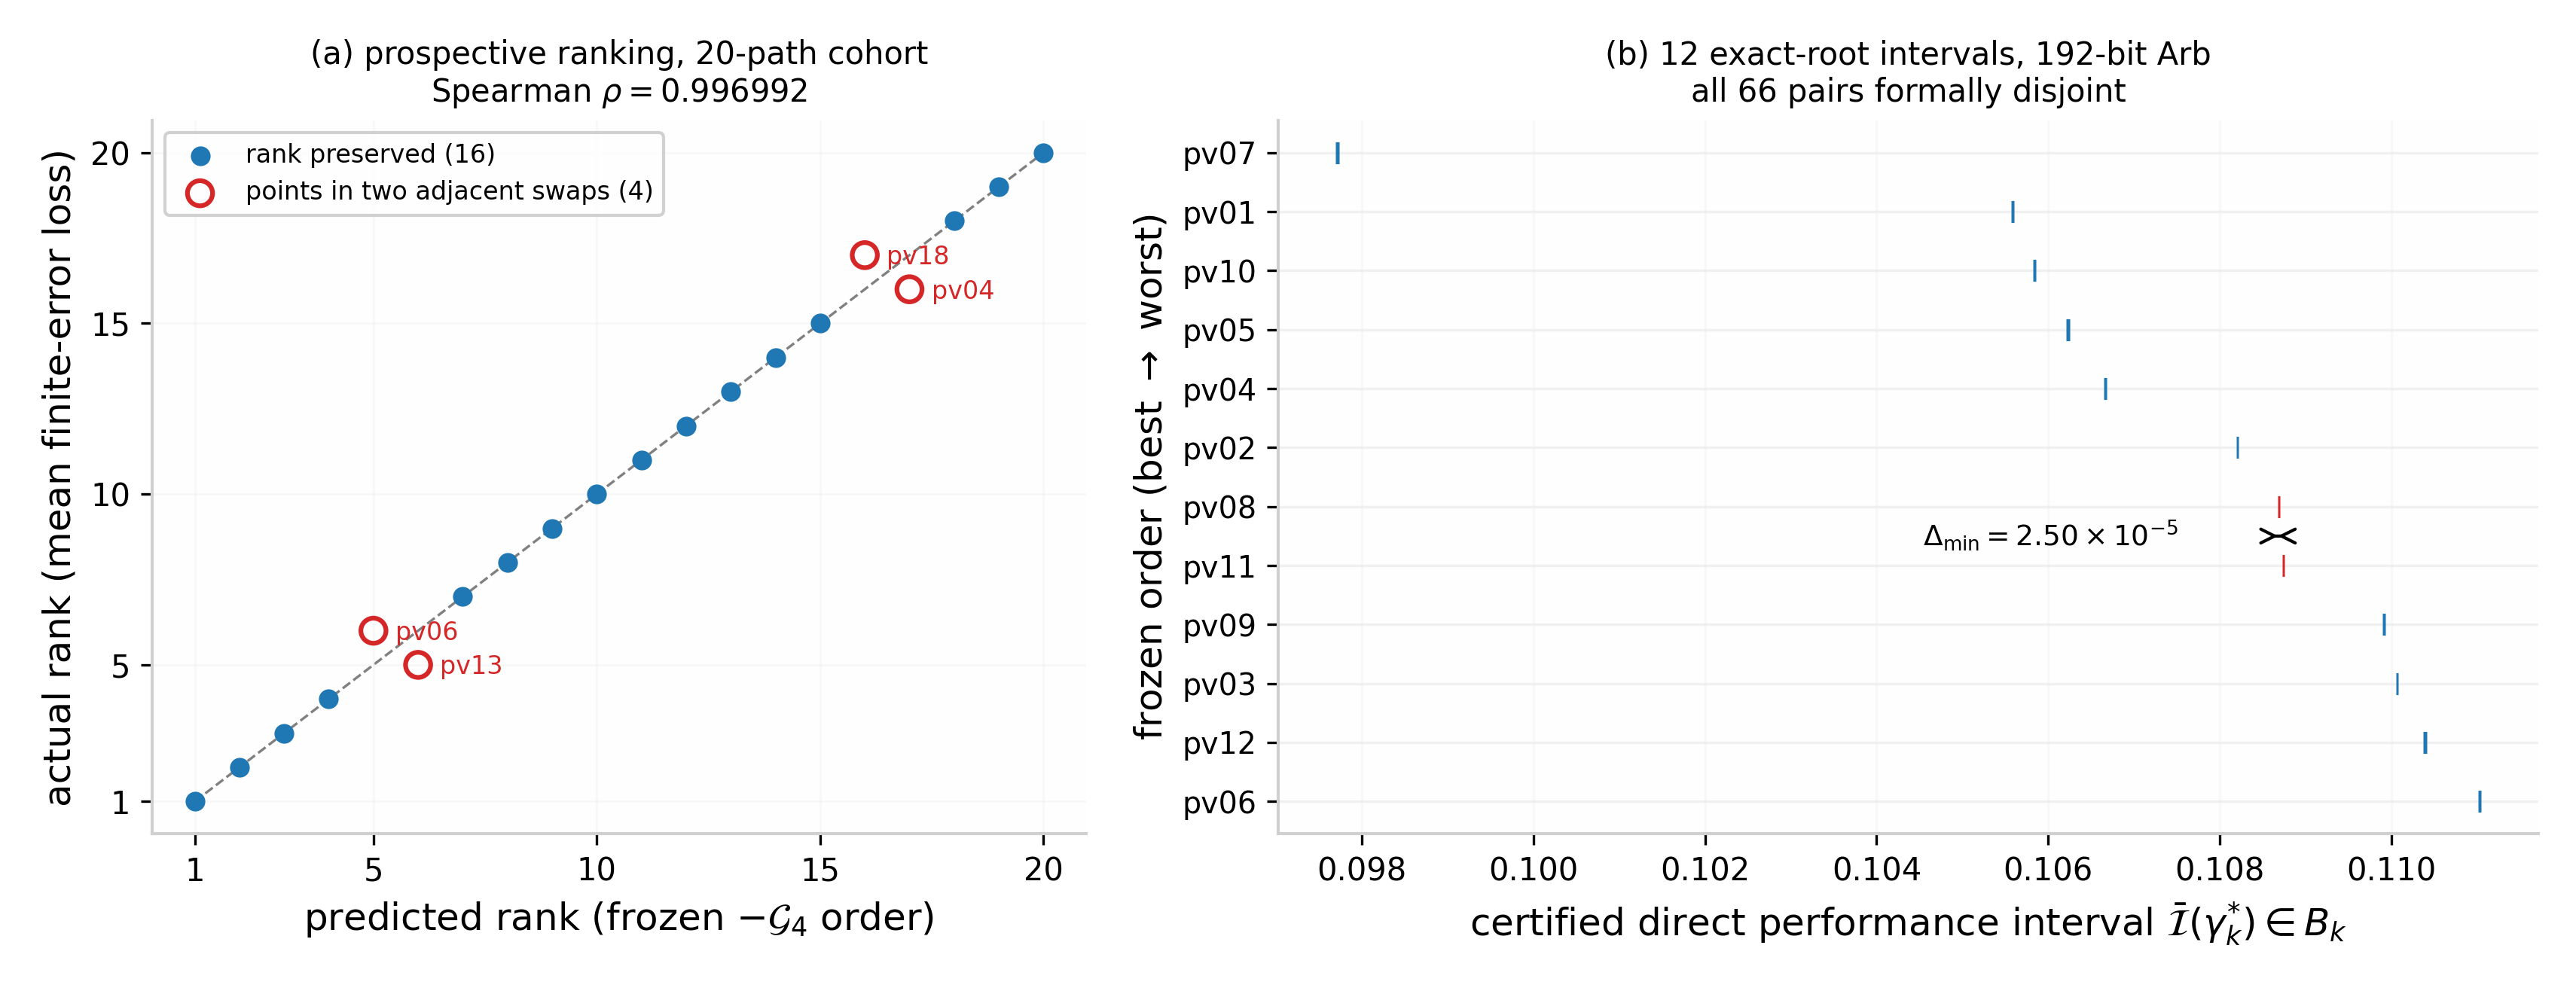
\includegraphics[width=0.95\textwidth]{fig2.png}
\caption{Direct visual evidence for the two claims in the title. (a) Prospective
prediction: $-\Gg_{4}$ predicted versus actual ranks on the held-out twenty-path cohort.
The frozen order reproduces the actual mean-loss ranking up to two adjacent transpositions
(marked), giving Spearman $\rho=0.996992$. This panel reports prospective empirical
evidence; it is not a certificate. (b) Exact-root certification: the twelve certified
direct performance intervals $B_{k}$ from 192-bit outward-rounded Arb propagation, drawn to
scale in the frozen order. All 66 unordered pairs are formally disjoint; the tightest pair,
pv08--pv11, has the certified margin $\Delta_{\min}=2.50\times10^{-5}$ of
Corollary~\ref{cor:stability} (inset: magnification of that pair).}
\label{fig:evidence}
\end{figure}

\section{Discussion}\label{sec:discussion}

\subsection{Why the quartic term is useful but incomplete}

First-order matching makes the quadratic loss nearly common---exactly common at exact
matched roots by Lemma~\ref{lem:quadratic}. This promotes the quartic term to the first
visible discriminator. It explains why $\Gg_{4}$ often gives almost perfect rankings.
However, if two quartic coefficients are close, the sixth and higher terms can reverse
their order. The formal intervals expose this distinction directly: 34 pairs are
quartic-certified, while the remaining pairs require higher jet data or direct propagation.

This is preferable to declaring the quartic rule either universally true or false. The
correct statement is gap-dependent as in Eq.~\eqref{eq:gaptest}.

\subsection{Minimal model versus scalable certification}

The role of the two-atom model is to isolate the response-matching mechanism in the
smallest interacting Rydberg system, not to approximate a many-body processor. The present
certificate shows that residual finite-error ordering survives exact projective state and
complete first-response matching without being attributable to optimizer residuals. Turning
this result into a many-body compilation method requires a separate scalability programme,
including structured state representations and dependency-preserving validated propagation.
The current theorem should therefore be read as a minimal rigorous existence-and-ordering
result rather than as a scalable hardware-design algorithm.

\subsection{Order-30 mechanism versus direct propagation}

The order-30 jet propagated over the Krawczyk boxes certifies 52/66 pairs with zero
reversals (Proposition~\ref{prop:order30}). The remaining 14 pairs are not physically
reversed---they are unresolved due to dependency and wrapping in the phase-box propagation
of the jet enclosure. Direct Arb propagation of the same boxes certifies all 66 pairs
(Theorem~\ref{thm:ordering}), demonstrating that the unresolved cases are an artefact of
the jet propagation and interval wrapping, not a physical failure of the frozen ordering.
The 52/66 mechanism certificate and the 66/66 direct certificate arise from different
propagation levels and should not be conflated: the latter is the main theorem.

The content is quantitative rather than existential: an analytic finite-dimensional
propagator is determined by its local germ, but here a fixed finite order, 30, resolves
52/66 comparisons with an explicitly bounded tail, and the unresolved cases arise from
interval wrapping rather than truncation.

The particular ordering of the twelve serialized controls is not presented as a universal
physical law. The reusable contribution is the certificate architecture: transverse
exact-root isolation, formal propagation of the resulting root boxes, and explicit
separation between low-order mechanism certificates and direct finite-error theorems.

\section{Limitations and next theorem}\label{sec:limitations}

The present work has five explicit limitations.
\begin{enumerate}[itemsep=0.15em]
\item \textbf{Global fibre structure.} Twelve locally unique roots exactly matched in
projective output state and first projective response are certified in transverse boxes.
The global eight-dimensional solution manifold structure remains unproved.
\item \textbf{Finite-dimensional model.} Spontaneous emission, Doppler effects, laser phase
noise, position fluctuations, leakage levels, and waveform filtering are absent. An
open-system extension is not obtained by appending a dissipative curve to the present
certificate. Exact matching of density matrices or quantum channels and their first
responses defines a different constraint map, whose dimension generally scales with
$d^{2}$ rather than $d$. It would require new matched controls, new root boxes, and
validated Liouvillian propagation. Arbitrary dissipative perturbations need not preserve
the present ordering, and no noise-model-independent ordering theorem is claimed here.
\item \textbf{Two atoms.} No many-body scaling theorem is claimed.
\item \textbf{Mean axial error law.} The primary result concerns the declared six-axis
mean. Worst-case ranking is not supported by the present scalar.
\item \textbf{No QPU evidence.} The calculations are local and require no hardware access.
They do not constitute physical-QPU evidence.
\end{enumerate}
In short, the certificate is formal for the serialized finite-dimensional two-atom
Hamiltonian, the declared transverse boxes, and the six-axis mean error functional; it does
not certify model discrepancy, global fibre topology, many-body scaling, or hardware.

\subsection{Constraint dimension and scalability}

The present dense interval implementation is not a scalable many-body compiler. Its
dimensional growth can nevertheless be stated explicitly. Suppose the reachable complex
state space has dimension $d$, and let $m$ be the number of calibrated error coordinates.
Matching one projective output state and its $m$ complete projective first responses
imposes
\[
q=2(m+1)(d-1)
\]
real projective constraints. When the constraint Jacobian has rank $q$, a square Krawczyk
chart uses $q$ transverse control variables, while any remaining independent control
variables parameterize numerical fibre directions.

Here $m=3$ and the exchange-symmetric two-atom state space has $d=3$, giving
\[
q=2(3+1)(3-1)=16,
\]
with $24-16=8$ numerical fibre directions. For a fully permutation-symmetric $N$-atom
two-level model, $d=N+1$ and the corresponding constraint count is $8N$. For a generic
unsymmetrized model, $d=2^{N}$ and the dense constraint count becomes $8(2^{N}-1)$.

Thus exponential growth is not intrinsic to the Krawczyk operator alone; it arises through
the dimension of the reachable state representation and the cost of enclosing the
associated propagators and Jacobians. In generic many-body settings, direct dense Arb/ACB
propagation and naive interval Jacobians would also suffer rapidly increasing dependency
and wrapping. Possible routes to larger systems include symmetry reduction, sparse or
block-structured propagation, reduced-observable matching, tensor-network enclosures,
Taylor or Chebyshev polynomial models with validated remainder bounds, interval
subdivision, and parameter-dependent Krawczyk charts. Taylor or Chebyshev polynomial models
with validated remainder bounds may help reduce local propagation overestimation, but they
do not by themselves remove the exponential growth of a generic many-body state
representation. None of these extensions is implemented or certified in the present work.

The next mathematical step is a validated implicit-function theorem or a
parameter-dependent Krawczyk atlas: treat the eight fibre coordinates as parameters and
certify a unique transverse solution varying over a declared fibre neighbourhood. The
target mathematical structure is
\[
F(x,y)=0,\qquad x\in\Rr^{16},\ y\in\Rr^{8},
\]
and the goal is to prove that a unique transverse solution $x=x(y)$ exists and is regular
over a declared $y$-region, not to prove a single global isolated root.

\section{Reproducibility}\label{sec:repro}

The complete formal pipeline is frozen in a single standalone audit (v1.3). The
twelve-path cohort, the transverse bases, and the point preconditioners are fixed; the
common Krawczyk radius is $3\times10^{-12}$; and runtime metadata is excluded from every
hashed proof object. Two complete formal executions produce byte-identical protocol,
certificate, and report files. The SHA-256 certificate identifiers and the numerical
integrity diagnostics are collected in Appendix~\ref{app:hashes}; the script inventory,
dependency pins, and clean-environment runs are collected in Appendix~\ref{app:scripts}.

\textbf{Clean-environment reproduction.} The complete v1.3 audit was rerun in a clean
external Colab environment from the public v0.3.1 Git tag, which resolved to commit
\begin{center}
\footnotesize\texttt{284974c9f6b952f4e114c8c5bdc9c2c299c4065c}.
\end{center}
Dependency installation, repository
SHA-256 verification, reference-artifact validation, regression tests, and the complete
two-run formal recomputation all passed. The run required no vendor account or cloud
credentials.

\section{Conclusion}\label{sec:conclusion}

We establish two complementary results on distinct frozen cohorts. On a prospective
twenty-path cohort, the zero-point quartic geometric scalar strongly predicts held-out
finite-error performance. On a separate twelve-path formal cohort, direct outward-rounded
interval propagation certifies all 66 pairwise finite-error orderings at locally unique
roots exactly matched in projective output state and first projective response.

The common endpoint and complete first-order state response leave residual path dependence.
A coordinate-covariant fourth-order response tensor provides a strong and partially
certifying low-order description, but close comparisons require higher derivatives. On the
twelve-path cohort, strict Krawczyk inclusions establish the twelve locally unique exact
roots. The zero-error jet through order thirty, combined with rigorous Cauchy-alias and
Dyson-tail enclosures, certifies 52/66 exact-root comparisons with zero reversals as a
separate mechanism certificate. Direct 192-bit outward-rounded Arb propagation of the
Krawczyk boxes certifies all 66 pairwise orderings as the main theorem.

The explicit constraint-dimension count identifies the boundary of the present dense
certificate: it remains tractable in the minimal interacting model and in suitably reduced
symmetry sectors, but no generic many-body scalability claim is made. The next steps are
parameterized root continuation, certified model-discrepancy budgets, structured many-body
propagation, and separate open-system and compiled-hardware validation.

\appendix

\section{Interval-arithmetic certificate construction}\label{app:interval}

For completeness we collect the construction parameters of the formal certificates. All
formal objects are computed in 192-bit outward-rounded Arb/ACB ball
arithmetic~\cite{johansson2017}: every phase-dependent trigonometric factor, Hamiltonian
matrix exponential, state propagation, overlap, infidelity, and six-point mean is enclosed.
For each declared path, the Krawczyk computation uses a point preconditioner given by a
numerical inverse of the midpoint Jacobian, a common transverse box radius of
$3\times10^{-12}$, an interval enclosure of the Jacobian over the full box, and the strict
inclusion test $K(X)\subset\intt(X)$; the projective chart denominator $\psi_{0}$ is
verified to exclude zero on every accepted box. The order-thirty mechanism certificate
extracts Taylor coefficients by a 64-point outward-rounded Cauchy discrete Fourier
transform; the discrete-transform alias is enclosed by the path-uniform Dyson bound
$e^{K_{a}}K_{a}^{64}/64!<10^{-40}$ on every physical error axis, and the analytic even
Dyson tail after order thirty is enclosed by $2\times10^{-11}$. As an integrity diagnostic,
every ordinary held-out floating-point outcome is verified to lie inside its corresponding
formal ball; this diagnostic is not part of the theorem proofs.

\section{Certificate identifiers and integrity diagnostics}\label{app:hashes}

The frozen twelve-path cohort hash is
\begin{center}
\footnotesize\texttt{9942af610c1e9499a10e989e4ae069e3}\\
\footnotesize\texttt{912d58eec4fd3ad1d3d39947c232c356}.
\end{center}
The deterministic protocol and certificate hashes are:
\begin{itemize}[itemsep=0.1em]
\item Krawczyk protocol:\\
\footnotesize\texttt{a19d01ec77a783be4e3858dd92ca080a}\\
\footnotesize\texttt{a9fde2b09b77541b0e1ad7f392ff3124}
\item Krawczyk certificate:\\
\footnotesize\texttt{fc3ad3823597bd5281b7b9292f227f72}\\
\footnotesize\texttt{3c2b3a9a8aa4e42c9f0353921b4d8fec}
\item Exact-root ordering protocol:\\
\footnotesize\texttt{f51ecfd2e4572f271e276cae18697005}\\
\footnotesize\texttt{baa3f0ec3f3ab94f98f919cd50c3f844}
\item Exact-root ordering certificate:\\
\footnotesize\texttt{03c4db75cb80a149ce1a61e11c227039}\\
\footnotesize\texttt{f9bd79c3f1304b3defa311a491ea2d1e}.
\end{itemize}

\begin{table}[htbp]
\centering
\caption{Numerical integrity diagnostics from representative Colab runs.}
\label{tab:integrity}
\small
\begin{tabular}{@{}ll@{}}
\toprule
Diagnostic & Value\\
\midrule
Fourth-tensor independent components & 15\\
Maximum tensor recovery relative residual & $4.63\times10^{-15}$\\
Direct coordinate-refit relative error & $1.08\times10^{-14}$\\
Invariant-contraction relative error & $2.36\times10^{-15}$\\
Quadratic-coefficient relative spread & $1.09\times10^{-7}$\\
Arb precision & 192 bits\\
Cauchy points & 64\\
Taylor order & 30\\
Formal quartic pair coverage & $34/66=51.52\%$\\
Exact-root order-30 mechanism coverage & $52/66=78.79\%$\\
Exact-root direct Arb ordering coverage & $66/66=100\%$\\
\bottomrule
\end{tabular}
\end{table}

\section{Scripts and clean-environment reproduction}\label{app:scripts}

The principal standalone scripts are:
\begin{center}
\footnotesize\texttt{pasqal\_two\_atom\_G4\_standalone\_colab.py}\\
\footnotesize\texttt{pasqal\_L3\_L4\_standalone\_colab.py}\\
\footnotesize\texttt{pasqal\_L4\_order30\_standalone\_colab.py}\\
\footnotesize\texttt{pasqal\_L4\_formal\_arb\_standalone\_colab.py}\\
\footnotesize\texttt{pasqal\_L4\_exact\_fibre\_krawczyk\_standalone\_colab\_v1\_2.py}\\
\footnotesize\texttt{pasqal\_L4\_exact\_root\_ordering\_standalone\_colab.py}\\
\footnotesize\texttt{pasqal\_L4\_reproducible\_certificate\_v1\_3\_colab.py}
\end{center}
The last script produces all formal proof objects. The formal standalone script pins
\texttt{python-flint==0.8.0}. NumPy and SciPy provide numerical diagnostics, while the
v1.3 proof consumes the frozen decimal cohort and uses Arb/ACB for the formal interval
certificate.

Two independent clean-environment Colab executions of the complete v1.3 audit, started from
the public v0.3.1 tag, completed in 52.6 s and 107.9 s respectively; in both runs,
dependency installation, repository SHA-256 verification, reference-artifact validation,
regression tests, and the two-run byte-identical formal recomputation passed.

\section*{Code and Data Availability}
All code, frozen inputs, formal certificates, and reproduction scripts are available at
\begin{center}
\url{https://github.com/papasop/quantum-control-geometry}
\end{center}
The formal computational artifacts used in this work are fixed in release v0.3.1 at commit
\begin{center}
\footnotesize\texttt{284974c9f6b952f4e114c8c5bdc9c2c299c4065c}.
\end{center}
The synchronized manuscript source is
maintained on the repository's \texttt{main} branch. No PASQAL account or cloud credentials
are required.

\section*{Funding}
The author received no external funding for this work.

\section*{Competing Interests}
The author declares no competing interests.

\section*{Author Contributions}
Y.Y.N.Li conceived the study, developed the theoretical framework, implemented the
numerical and formal audits, analyzed the results, and wrote the manuscript.

\begin{thebibliography}{20}\small\raggedright\sloppy

\bibitem{silverio2022pulser}
H.~Silv\'erio, S.~Grijalva, C.~Dalyac, L.~Leclerc, P.-J.~Karalekas, N.~Shammah, M.~Beji,
L.-P.~Henry, and L.~Henriet, ``Pulser: An open-source package for the design of pulse
sequences in programmable neutral-atom arrays,'' \emph{Quantum} \textbf{6}, 629 (2022).
doi:10.22331/q-2022-01-24-629.

\bibitem{henriet2020}
L.~Henriet, L.~Beguin, A.~Signoles, T.~Lahaye, A.~Browaeys, G.-O.~Reymond, and
C.~Jurczak, ``Quantum computing with neutral atoms,'' \emph{Quantum} \textbf{4}, 327
(2020). doi:10.22331/q-2020-09-21-327.

\bibitem{saffman2016}
M.~Saffman, ``Quantum computing with atomic qubits and Rydberg interactions: progress and
challenges,'' \emph{J.~Phys.~B: At.~Mol.~Opt.~Phys.} \textbf{49}, 202001 (2016).
doi:10.1088/0953-4075/49/20/202001.

\bibitem{wimperis1994}
S.~Wimperis, ``Broadband, narrowband, and passband composite pulses for use in advanced
NMR experiments,'' \emph{J.~Magn.~Reson.~A} \textbf{109}, 221--231 (1994).
doi:10.1006/jmra.1994.1159.

\bibitem{kukita2022}
S.~Kukita, H.~Kiya, and Y.~Kondo, ``General off-resonance-error-robust symmetric composite
pulses with three elementary operations,'' \emph{Phys.~Rev.~A} \textbf{106}, 042613 (2022).
doi:10.1103/PhysRevA.106.042613.

\bibitem{barnes2015}
E.~Barnes, X.~Wang, and S.~Das~Sarma, ``Robust quantum control using smooth pulses and
topological winding,'' \emph{Sci.~Rep.} \textbf{5}, 12685 (2015). doi:10.1038/srep12685.

\bibitem{johansson2017}
F.~Johansson, ``Arb: Efficient arbitrary-precision midpoint-radius interval arithmetic,''
\emph{IEEE Trans.~Comput.} \textbf{66}, 1281--1292 (2017). doi:10.1109/TC.2017.269063.

\bibitem{dyson1949}
F.~J.~Dyson, ``The radiation theories of Tomonaga, Schwinger, and Feynman,''
\emph{Phys.~Rev.} \textbf{75}, 486--502 (1949). doi:10.1103/PhysRev.75.486.

\bibitem{tucker2011}
W.~Tucker, \emph{Validated Numerics: A Short Introduction to Rigorous Computations},
Princeton University Press, Princeton (2011).

\bibitem{tucker2002}
W.~Tucker, ``A rigorous ODE solver and Smale's 14th problem,'' \emph{Found.~Comput.~Math.}
\textbf{2}, 53--117 (2002). doi:10.1007/s002080010018.

\bibitem{lanford1982}
O.~E.~Lanford, ``A computer-assisted proof of the Feigenbaum conjectures,''
\emph{Bull.~Amer.~Math.~Soc.} \textbf{6}, 427--434 (1982).
doi:10.1090/S0273-0979-1982-15008-X.

\bibitem{vandenberg2015}
J.~B.~van~den~Berg and J.-P.~Lessard, ``Rigorous numerics in dynamics,''
\emph{Notices Amer.~Math.~Soc.} \textbf{62}, 1057--1061 (2015). doi:10.1090/noti1276.

\bibitem{rabitz2004}
H.~A.~Rabitz, M.~M.~Hsieh, and C.~M.~Rosenthal, ``Quantum optimally controlled transition
landscapes,'' \emph{Science} \textbf{303}, 1998--2001 (2004). doi:10.1126/science.1093649.

\bibitem{chakrabarti2007}
R.~Chakrabarti and H.~Rabitz, ``Quantum control landscapes,'' \emph{Int.~Rev.~Phys.~Chem.}
\textbf{26}, 671--735 (2007). doi:10.1080/01442350701633300.

\bibitem{khaneja2005}
N.~Khaneja, T.~Reiss, C.~Kehlet, T.~Schulte-Herbr\"uggen, and S.~J.~Glaser, ``Optimal
control of coupled spin dynamics: design of NMR pulse sequences by gradient ascent
algorithms,'' \emph{J.~Magn.~Reson.} \textbf{172}, 296--305 (2005).
doi:10.1016/j.jmr.2004.11.004.

\bibitem{vandersypen2005}
L.~M.~K.~Vandersypen and I.~L.~Chuang, ``NMR techniques for quantum control and
computation,'' \emph{Rev.~Mod.~Phys.} \textbf{76}, 1037--1069 (2005).
doi:10.1103/RevModPhys.76.1037.

\bibitem{green2013}
T.~J.~Green, J.~Sastrawan, H.~Uys, and M.~J.~Biercuk, ``Arbitrary quantum control of
qubits in the presence of universal noise,'' \emph{New J.~Phys.} \textbf{15}, 095004
(2013). doi:10.1088/1367-2630/15/9/095004.

\bibitem{khodjasteh2009}
K.~Khodjasteh and L.~Viola, ``Dynamically error-corrected gates for universal quantum
computation,'' \emph{Phys.~Rev.~Lett.} \textbf{102}, 080501 (2009).
doi:10.1103/PhysRevLett.102.080501.

\bibitem{provost1980}
J.~P.~Provost and G.~Vallee, ``Riemannian structure on manifolds of quantum states,''
\emph{Commun.~Math.~Phys.} \textbf{76}, 289--301 (1980). doi:10.1007/BF02193559.

\bibitem{moore2009}
R.~E.~Moore, R.~B.~Kearfott, and M.~J.~Cloud, \emph{Introduction to Interval Analysis},
SIAM, Philadelphia (2009).

\end{thebibliography}
